\chapter{Java 8}

\section{default \& statische Methoden für Interfaces}

Vor Java 8 beschrieben Interfaces nur Schnittstellen und hatten auf keinen Fall eine Implementierung. In Java 8 können Interfaces nun mit statischen- und default-Methoden, Implementierungen beinhalten. Interfaces sind jetzt ganz ähnlich wie abstrakte Klassen, haben aber keinen Zustand und auch keinen Konstruktor. Es kann zudem nur eine abstrakte Klasse beerbt werden, aber es können mehrere Interfaces implementiert werden. Die Hauptmotivation für diese Neuerung war die \textbf{Rückwärtskompatibilität}. Die statischen-Methoden müssen im Interface implementiert werden und können von den implementierenden Klassen nicht überschrieben werden \textit{(in PHP möglich)}. Zudem muss der Aufruf der statischen-Methoden direkt über die Interfaces laufen. Durch default-Methoden lassen sich bestehende Interfaces erweitern, ohne bestehende Implementierungen zu brechen (\textit{defender methods}). Als Beispiel wurde das \verb|Collection|-Interface um eine \verb|stream()|-Methode erweitert. Da eine Klasse mehrere Interfaces implementieren kann, kann es zu Konflikten kommen, wenn es zwei Interfaces mit gleicher default-Methode gibt. Die betroffene Methode muss dann in der Klasse explizit überschrieben werden. Listing \ref{lst:default-statische-methoden} zeigt die beiden Methoden in einem Beispiel.

\begin{lstlisting}[language=Java, caption=Default- und statische Methoden, label=lst:default-statische-methoden]
public interface DemoInterface {
	default int getLuckyNumber() { return 7; }
	static int getEight() { return 8; }
}

int eight = DemoInterface.getEight();
DemoInterface di = new DemoInterface() {};
int seven = di.getLuckyNumber();

public interface OtherInterface {
	default int getLuckyNumber() { return 8; }
}

public class InterfaceDemo implements DemoInterface, OtherInterface {
	@Override
	public int getLuckyNumber() {
		// Neuer super syntax. Der Aufruf einer Interface-Default-Methode von einer implementierende Klasse aus, muss so erfolgen. Der folgende Aufruf, ausserhalb einer implementieren Klasse, funktioniert nicht.
		return DemoInterface.super.getLuckyNumber();
	} 
}
\end{lstlisting}

\section{Lambda-Ausdrücke}

Mit Java 8 wurden neu Lambdas (oder nach Java-Slang: Closure) eingeführt. Listing \ref{lst:lambda-ausdruecke} zeigt die Syntax. \textit{Lambdas sind: anonyme Methoden (ad-hoc Implementationen), code as data - first class citizen (Funktioanlität als Parameter/Rückgabewert) und überlegen gegnüber (anonymen) inneren Klassen.}

\begin{lstlisting}[language=Java, caption=Lambda-Ausdrücke, label=lst:lambda-ausdruecke]
(int x, int y) -> { return x+y; }

// Argument type is inferred:
(x, y) -> { return x+y; }

// No brackets needed if only one argument
x -> { return x+1; }

// No arguments needed
() -> { System.out.println("I am a Runnable"); }

// Lambda using a statement block
a -> {
	if (a.balance() < limit) a.alert();
	else a.okay();
}

// Single expression
a -> (a.balance() < limit) ? a.alert() : a.okay()

// returns Account
(Account a) -> { return a; }

// returns int
() -> 5;
\end{lstlisting}

Der Typ eines Lambdas ist ein \textit{Funktionales Interface}. Ein Lambda kann auch als Interface-Instanz betrachtet werden. Ein funktionales Interface ist ein Interface mit einer Methode (Single Abstract Methode - SAM) und der optionalen Annotation \verb|@FunctionalInterface|. Listing \ref{lst:functional-interface} zeigt ein Beispiel für ein funktionales Interface.

\begin{lstlisting}[language=Java, caption=functional interface (SAM), label=lst:functional-interface]
@FunctionalInterface // annotation is optional
interface Consumer<T> {
	void accept(T a);
}

Consumer<Account> myLambda = (Account a) -> {if (a.balance() < limit) a.alert(); };
\end{lstlisting}

Java bringt eine vorgegebene Sammlung von funktionalen Interfaces mit, welche in folgende Typen unterteilt sind:
\begin{description}
	\item[Consumer:] Produziert kein Resultat (keine Rückgabe)
	\item[Function:] Produziert Resultat von beliebigem Typ
	\item[Operator:] Produziert Resultat vom Argument-Typ
	\item[Supplier:] Produziert Resultat ohne Argument
	\item[Predicate:] Produziert boolean-Resultat
\end{description}
Zusätzlich gibt es noch folgende Namensregeln:
\begin{itemize}
	\item Präfix \textit{Bi} falls zwei Argumente, \textit{Binary} bei Operator (z.B.: \verb|BiPredicate<T, U>|, \verb|BinaryOperator<T>|
	\item Präfix \textit{Unary} falls Operator mit einem Argument (z.B.: \verb|UnaryOperator<T>|)
	\item Elementare Datentypen kommen im Namen vor (z.B. \verb|DoublePredicate|)
	\item Funktionen mit unterschiedlichen elementaren Argument- und Resultat-Typen benutzen \textit{To}-Notation (z.B. \verb|IntToLongFunction|
\end{itemize}
Generics definieren je nachdem Argument-Typen und/oder Rückgabe-Typ. Lambdas führen keinen neuen Scope ein und haben dadurch Zugriff auf lokale Variablen vom umschliessenden Scope. Diese Variablen müssen aber \textit{effectively final} sein d.h. nach der ersten Zuweisung dürfen sie nicht mehr verändert werden. Die Anwendung des \verb|final| Schlüsselworts ist nicht zwingend. 

Mittels Methoden-Referenzen (z.B. \verb|String::length|) können existierende Methoden einer Klasse als Lambda-Ausdrücke verwendet werden. Dadurch kann im Gegensatz zu Lambdas weniger Code geschrieben werden und dieser auch wiederverwendet werden. Es gibt die folgenden vier Typen von Methoden-Referenzen:
\begin{itemize}
	\item Statische Methode: \verb|System::currentTimeMillis|
	\item Instanzmethode eines Objektes: \verb|System.out::println|
	\item Instanzmethode einer bel. Instanz einer gewissen Klasse: \verb|String::length|
	\item Konstruktor: \verb|String::new|
\end{itemize}
Mit Lambdas lassen sich dann tolle Dinge anstellen wie Event-Listener oder Runnables kompakt zu implementieren. \\

\textit{Bei \textbf{Lexical Scoping} ist die Sichtbarkeit von Variabeln durch den Programm-Code vorgegeben. Wobei die Variablen im selben und in darunterliegenden Blöcken sichtbar sind. Dies kann zur Kompilierzeit (early binding) ermittelt werden. Dies wird in den meisten Sprachen so gemacht - auch in Java. Alternativ gibt es das \textbf{dynamic Scoping}, wobei die Sichtbarkeit vom Ausführungs- bzw. Aufruf-Kontext abhängt. Das wird erst zur Laufzeit bestimmt (late binding). Oft in LISP-Sprachen wie Perl gesehen.}

\section{Streams}

Mit Java 8 wurde ein neue Datenstruktur Stream eingeführt, welche es ermöglicht Funktionen elegant auf Datenstrukturen anzuwenden. Dadurch stehen in Java Funktionen höherer Ordnung (\textit{higher order functions}) zur Verfügung, welche als Argument ein Lambda-Ausdruck entgegennehmen. Nachfolgend einige Beispiele dieser neuen \textit{Aggregate Operations (aka Bulk Operations)}:
\begin{description}
	\item[for-each:] Funktionalität auf jedes Element anwenden (z.B. \verb|accounts.forEach(a -> a.addInterest());|)
	\item[filter:] Neue Sequenz erstellen aus den Resultaten, wenn auf jedes originale Element ein Filter angewandt wurde (z.B. \verb|accounts.filter(a -> a.balance() > 1_000_000 );|)
	\item[map:] Neue Sequenz erstellen aus den Resultaten, wenn auf jedes originale Element eine Abbildung angewandt wurde. (z.B. \verb|accounts.map(a -> a.balance());|)
	\item[reduce:] Produziert einzelnes Resultat aus allen Elementen (z.B. \verb|accounts.map(a -> a.balance()).reduce(0, (b1, b2) -> b1+b2);|)
\end{description}
Neben dem generischen Stream gibt es aus Performance-Gründen auch Streams für diese drei primitiven Datentypen, welche direkt von \verb|BaseStream| erben:
\begin{itemize}
	\item \verb|IntStream| (Diesen für \verb|char| nehmen)
	\item \verb|DoubleStream| (Diesen für \verb|float| nehmen)
	\item \verb|LongStream|
\end{itemize}
Um einen Stream zu bekommen kann man z.B. die \verb|stream()|-Methode des \verb|Collection|-Interfaces aufrufen oder eine statische Factory-Methode eines Stream-Interfaces benutzen (z.B. \verb|range()| von \verb|IntStream|). Stream-Operationen wie \verb|filter()|, \verb|map()| usw. produzieren wieder einen Stream \textbf{(intermediate/lazy)} und werden erst ausgewertet wenn sie wirklich gebraucht werden. Stream-Operationen wie \verb|forEach()|, \verb|reduce()| usw. produzieren keinen neuen Stream \textbf{(terminal/eager)} sondern werten die intermediate-Streams zu einem Resultat aus. Nach dem Aufruf einer terminal-Operation ist der Stream \textit{aufgebraucht}, es kann also nur eine terminal-Operation pro Stream aufgerufen werden. Dass intermediate-Streams nicht sofort ausgewertet werden hat einen positiven Einfluss auf die Performance. 

Bei der \verb|reduce()|-Methode muss immer eine \textit{Identity} mitgegeben werden. Die Identity sollte dass Resultat einer Funktion nicht verändern (neutraler Wert). Möchte man z.B. einen \verb|IntStream| summieren, wäre die Identity 0 weil 0 das Resultat nicht verändert (z.B. 3 + 0 = 3). Listing \ref{lst:stream} zeigt einen Stream, welcher in fluent Programming definiert wurde.

\begin{lstlisting}[language=Java, caption=Stream, label=lst:stream]
int sum = widgets.stream()
	.filter(w -> w.getColor() == RED)
	.mapToInt(w -> w.getWeight())
	.sum();
\end{lstlisting}

Bei den intermediate Operations wird zwischen \textbf{stateless} (z.B. \verb|filter()|, \verb|map()|) und \textbf{stateful} Operations (z.B. \verb|limit()|, \verb|sorted()|) unterschieden. Bei stateless Operations wird nur das aktuelle Element verwendet, dadurch sind diese einfach handhabbar. Bei stateful Operation wird nebst dem aktuellen Element auch ein Zustand benötigt, dadurch müssen Resultate zwischengespeichert werden und der Stream mehrmals durchlaufen werden. Dies erschwert die Parallelisierung. \verb|sorted()| ist die komplexeste und restriktivste stateful operation. 

Ausserdem gibt es \textit{short-circuiting Operations}, welche die Abarbeitung stoppen können, bevor das letzte Element erreicht ist. Dabei wird wieder zwischen intermediate (z.B. \verb|limit()|, \verb|skip()|) und terminal Operations (z.B. \verb|anyMatch()|, \verb|findFirst()|) unterschieden.

Streams lassen sich relativ einfach parallelisieren (z.B. mit der \verb|parallelStream()|-Methode des Collection-Interface). Dadurch werden Multi-Core-Rechner besser ausgenutzt ohne dass der Programmierer gross etwas davon merkt. Jeder sequentielle Stream kann in einen parallelen Stream umgewandelt werden, und umgekehrt. Gewisse Operationen verhalten sich bei sequentiellen Streams anders als bei parallelen Streams (z.B. stimmt Reihenfolge bei \verb|forEach()| nicht mehr). Die Lambdas die den Operationen auf einem parallelen Stream übergeben werden sollten zustandslos und non-interfering (Keine Änderung an der Stream-Quelle z.B. \verb|ArrayList| nicht verändern) sein.

Es lassen sich auch unendliche Streams (z.B. mit \verb|DoubleStream.generate(Math::random)|) generieren. Diese werden aber nicht direkt ausgewertet, weil es intermediate Opertions sind. Ein unendlicher Stream sollte unbedingt limitiert werden.

\begin{figure}[h!]
\centering
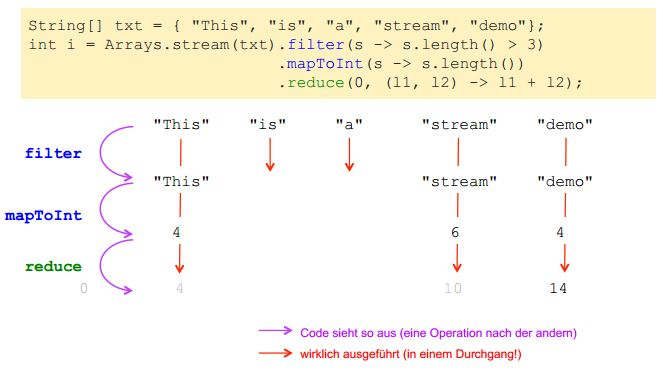
\includegraphics[width=0.4\linewidth]{fig/java-stream-executions}
\caption{Ausführungsreihenfolge in Streams}
\label{fig:java-stream-executions}
\end{figure}
